\setcounter{ExampleCounter}{1}
\marginnote{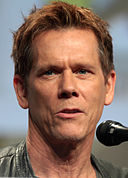
\includegraphics[width=1.5in]{KevinBacon}\\{\tiny\color{gray} CC BY-SA 2.0, Gage Skidmore}}
During a magazine interview in 1994, the actor Kevin Bacon made an offhand comment that he had ``worked with everybody in Hollywood or someone who's worked with them.''  From this sprang the idea of the \emph{Six Degrees of Kevin Bacon}, which sometimes appears as a game in which players must find a set of links between any given actor and Bacon.  For instance, Emma Watson has a Bacon number of 2, meaning that it takes two steps to get from her to Bacon (Watson was in \emph{The Circle} with Bill Paxton, who was in \emph{Apollo 13} with Kevin Bacon).

It turns out that, as the name suggests, a surprising number and range of actors can be connected to Kevin Bacon (or really any prolific actor) with six steps or fewer.  In fact, according to the website \emph{oracleofbacon.org}, there are over 1.2 million actors with a Bacon number of 4 or less, and the average Bacon number is just over 3.

\subsection{Paths and Circuits}

What we've described above is the process of finding the \textbf{shortest path} between two nodes on a graph (a graph where the nodes represent actors, and two nodes are connected by an edge if those two actors have appeared together).  We'll talk more about finding shortest paths in the next section, but for now, we can simply start with the definition of a \textbf{path}.

The definition of a path is quite intuitive: start at one node, then move along edges to another node, and you've taken a path.  We use the term \textbf{circuit} to describe a path that ends at the same node where it started (so a \emph{circuit} is a specific type of path; the term \emph{path} is a general one that includes circuits).
\begin{center}
\begin{tabular}{c c}
\begin{tikzpicture}
  \GraphInit[vstyle=simple]
  \tikzset{VertexStyle/.append style={scale=0.5}}
  \SetGraphUnit{1.4}
  
  \tikzset{VertexStyle/.append style={color=red}}
  \Vertex{1}
  \EA(1){2}
  \SO(1){4}
  \SOEA(1){5}
  \tikzset{VertexStyle/.append style={color=black}}
  \EA(2){3}
  \SO(3){6}

  \extralabel[2mm]{1}{135}{\color{red}$a$}
  \extralabel[2mm]{2}{90}{\color{red}$b$}
  \extralabel[2mm]{3}{45}{$c$}
  \extralabel[2mm]{4}{225}{\color{red}$d$}
  \extralabel[2mm]{5}{-90}{\color{red}$e$}
  \extralabel[2mm]{6}{-45}{$f$}
  
  \Edge(1)(2)
  \Edge(2)(3)
  \Edge(5)(6)
  \Edge(3)(6)
  \Edge(3)(5)
  \tikzset{EdgeStyle/.append style={color=red}}
  \tikzstyle{LabelStyle}=[color=red,fill=white]
  \Edge[label=1](1)(4)
  \Edge[label=2](4)(5) 
  \Edge[label=3](5)(2) 
  \Edge[label=4](2)(4)
\end{tikzpicture}
\hspace*{0.25in}
&
\hspace*{0.25in}
\begin{tikzpicture}
  \GraphInit[vstyle=simple]
  \tikzset{VertexStyle/.append style={scale=0.5}}
  \SetGraphUnit{1.4}
  
  \Vertex{1}
  \tikzset{VertexStyle/.append style={color=red}}
  \EA(1){2}
  \SO(1){4}
  \SOEA(1){5}
  \EA(2){3}
  \tikzset{VertexStyle/.append style={color=black}}
  \SO(3){6}

  \extralabel[2mm]{1}{135}{$a$}
  \extralabel[2mm]{2}{90}{\color{red}$b$}
  \extralabel[2mm]{3}{45}{\color{red}$c$}
  \extralabel[2mm]{4}{225}{\color{red}$d$}
  \extralabel[2mm]{5}{-90}{\color{red}$e$}
  \extralabel[2mm]{6}{-45}{$f$}
  
  \Edge(1)(2)
  \Edge(1)(4)
  \Edge(2)(3)
  \Edge(5)(6)
  \Edge(3)(6)
  \tikzset{EdgeStyle/.append style={color=red}}
  \tikzstyle{LabelStyle}=[color=red,fill=white]
  \Edge[label=1](2)(4)
  \Edge[label=2](4)(5)
  \Edge[label={3,4}](5)(3)
  \Edge[label=5](5)(2)
\end{tikzpicture}\\
& \\
\emph{Path:} $a \to d \to e \to b \to d$
\hspace*{0.25in}
&
\hspace*{0.25in}
\emph{Circuit:} $b \to d \to e \to c \to e \to b$
\end{tabular}
\end{center}

Note that in an undirected graph (like the two examples above), a path can travel in either direction along an edge, but in a directed graph, a path is only allowed to take an edge in its specified direction.

\begin{formula}{Paths and Circuits}
A \textbf{path} in a graph is a sequence of edges; if the graph is simple (no multiple edges between nodes), the path can be described using the nodes that it passes through in order.\\

A \textbf{circuit} is a path that starts and ends at the same node.
\end{formula}

Notice another distinction between the two graphs above: on the left, the path used four \emph{distinct} edges to travel from $a$ to $d$ (although the path passed through $d$ once before ending there), while the circuit on the right used the same edge (between $c$ and $e$) twice.  This brings us to another definition.

\begin{formula}{Simple Paths and Circuits}
A \textbf{simple} path or circuit is one that does not contain any edge more than once.
\end{formula}

In a moment, we'll return to the problem at the beginning of the last section: the K\"onigsberg Bridge Problem.  Remember that in that problem, we were hunting for a journey through the city that did not reuse any bridges; it turns out that we were actually looking for a \emph{simple path}.  Before we go back to that problem, though, we need to discuss one more concept: connectivity.
\pagebreak

\subsection{Connected Graphs}
A connected graph is exactly what you would expect:
\begin{center}
\begin{tabular}{c c}
\begin{tikzpicture}
  \GraphInit[vstyle=simple]
  \tikzset{VertexStyle/.append style={scale=0.5}}
  \SetGraphUnit{1.4}
  
  \Vertex{1}
  \EA(1){2}
  \EA(2){3}
  \EA(3){4}
  \SO(1){5}
  \SO(2){6}
  \SO(3){7}
  \SO(4){8}

  \extralabel[2mm]{1}{90}{$a$}
  \extralabel[2mm]{2}{90}{$b$}
  \extralabel[2mm]{3}{90}{$c$}
  \extralabel[2mm]{4}{90}{$d$}
  \extralabel[2mm]{5}{-90}{$e$}
  \extralabel[2mm]{6}{-90}{$f$}
  \extralabel[2mm]{7}{-90}{$g$}
  \extralabel[2mm]{8}{-90}{$h$}
  
  \Edge(1)(2)
  \Edge(2)(5)
  \Edge(5)(6)
  \Edge(2)(6)
  \Edge(6)(7)
  \Edge(3)(4)
  \Edge(3)(7)
  \Edge(3)(8)
  \Edge(4)(8)
\end{tikzpicture}
\hspace*{0.25in}
&
\hspace*{0.25in}
\begin{tikzpicture}
  \GraphInit[vstyle=simple]
  \tikzset{VertexStyle/.append style={scale=0.5}}
  \SetGraphUnit{1.4}
  
  \Vertex{1}
  \EA(1){2}
  \EA(2){3}
  \EA(3){4}
  \SO(1){5}
  \SO(2){6}
  \SO(3){7}
  \SO(4){8}

  \extralabel[2mm]{1}{90}{$a$}
  \extralabel[2mm]{2}{90}{$b$}
  \extralabel[2mm]{3}{90}{$c$}
  \extralabel[2mm]{4}{90}{$d$}
  \extralabel[2mm]{5}{-90}{$e$}
  \extralabel[2mm]{6}{-90}{$f$}
  \extralabel[2mm]{7}{-90}{$g$}
  \extralabel[2mm]{8}{-90}{$h$}
  
  \Edge(1)(2)
  \Edge(2)(5)
  \Edge(5)(6)
  \Edge(2)(6)
  \Edge(3)(4)
  \Edge(3)(7)
  \Edge(3)(8)
  \Edge(4)(8)
\end{tikzpicture}\\
& \\
\emph{Connected}
\hspace*{0.25in}
&
\hspace*{0.25in}
\emph{Disconnected}\\
& \hspace*{0.25in}
\emph{(with two connected components)}
\end{tabular}
\end{center}

The\marginnote{\emph{Note:} it's a bit more complicated for a directed graph; in that case, a graph is \emph{strongly connected} if there is an allowable path between every pair of vertices, and \emph{weakly connected} if we could find a path by ignoring directions.} definition is a simple one, and uses the idea of a path; a graph is connected if you can travel wherever you want from any starting place.

\begin{formula}{Connectivity}
An undirected graph is \textbf{connected} if there is a path between every pair of nodes in the graph.
\end{formula}

It turns out that we can even describe \emph{how} connected a graph is, by seeing how hard it is to make it disconnected (in the example above, it was pretty easy to do, by simply removing one edge).  But this simple description of connectivity is enough for us, because now we want to turn our attention back to the original problem: the bridges.

\subsection{Euler Paths}
Remember\marginnote{\includegraphics[width=1.5in]{Konigsberg}} the setup: we want to find a way to travel through the city of K\"onigsberg in such a way that we cross all of the seven bridges, but don't cross any more than once.  In other words, we want to find a \emph{simple path} through the following graph that uses every edge:
\begin{center}
\begin{tikzpicture}
  \GraphInit[vstyle=simple]
  \tikzset{VertexStyle/.append style={scale=0.5}}
  \SetGraphUnit{1.4}
  \Vertex{1}
  \NOWE(1){2}
  \SOWE(1){4}
  \WE(1){3}
  \Edge(1)(2)
  \Edge(1)(3)
  \Edge(1)(4)
  \SetUpEdge[style={bend right=30}]
  \Edge(2)(3)
  \Edge(3)(4)
  \SetUpEdge[style={bend left=30}]
  \Edge(2)(3)
  \Edge(3)(4)
\end{tikzpicture}
\end{center}

Just to clarify: a simple path means that we don't reuse edges, but we could leave some edges out.  The additional requirement that we use \emph{every} edge is what elevates this from a simple path to an \emph{Euler path}.

\begin{formula}{Euler Paths}
An \textbf{Euler path}\marginnote{Naturally, an Euler path is only possible in a connected graph.} in a graph is a path that goes through every edge of the graph exactly once.\\

\emph{Alternately, an Euler path is a simple path that contains every edge of the graph.}\\

An \emph{Euler circuit} is defined similarly: it is an Euler path that begins and ends at the same node.
\end{formula}

Now, the important question is, \emph{how can we tell if an Euler path or circuit is possible?}  If we know it's possible, of course, we'll also want to be able to find it.

It turns out that the answer to this question is surprisingly simple; there's something delightful about elegant answers like this one.  Let's see what Euler discovered; we'll take a look at a few examples to see what we can learn.
\pagebreak

Let's start with a simple one:
\begin{center}
\begin{tikzpicture}
  \GraphInit[vstyle=simple]
  \tikzset{VertexStyle/.append style={scale=0.5}}
  \SetGraphUnit{1.4}
  \Vertex{1}
  \SO(1){2}
  \WE(2){3}
  \SO(2){4}
  \WE(4){5}
  
  \Edge(1)(2)
  \Edge(1)(3)
  \Edge(2)(3)
  \Edge(2)(4)
  \Edge(2)(5)
  \Edge(4)(5)
\end{tikzpicture}
\end{center}

The goal is to trace over this graph, drawing every edge without lifting our virtual pen or retracing any lines.  With a little trial and error, we can find an Euler circuit; for instance, if we start at the top node, we can trace every edge and end up back at the same place:
\begin{center}
\begin{tikzpicture}
  \GraphInit[vstyle=simple]
  \tikzset{VertexStyle/.append style={scale=0.5}}
  \SetGraphUnit{1.4}
  \Vertex{1}
  \SO(1){2}
  \WE(2){3}
  \SO(2){4}
  \WE(4){5}
  
  \tikzset{EdgeStyle/.append style={color=red}}
  \tikzstyle{LabelStyle}=[color=red,fill=white]
  \Edge[label=1](1)(2)
  \Edge[label=6](1)(3)
  \Edge[label=5](2)(3)
  \Edge[label=2](2)(4)
  \Edge[label=4](2)(5)
  \Edge[label=3](4)(5)
\end{tikzpicture}
\end{center}

Notice\marginnote{\textbf{Observation 1:}\\ to draw an Euler circuit, every time we arrive at a node, there must be an unused edge we can use to leave.} that we can already draw one conclusion, in order to draw an Euler circuit, \emph{we can't get stranded anywhere}.  Now, what would it mean for us to get stranded?  If we can find an edge leading to a node, but there aren't any unused edges that we can use to leave, we'll be stuck.\\

While you mull on that, here's another example:
\begin{center}
\begin{tikzpicture}
  \GraphInit[vstyle=simple]
  \tikzset{VertexStyle/.append style={scale=0.5}}
  \SetGraphUnit{1.4}
  \Vertex{1}
  \EA(1){2}
  \SO(1){3}
  \EA(3){4}
  \SO(3){5}
  \EA(5){6}
  
  \extralabel{1}{135}{$a$}
  \extralabel{2}{45}{$b$}
  \extralabel{3}{180}{$c$}
  \extralabel{4}{0}{$d$}
  \extralabel{5}{225}{$e$}
  \extralabel{6}{-45}{$f$}
  
  \Edge(1)(2)
  \Edge(1)(3)
  \Edge(2)(3)
  \Edge(2)(4)
  \Edge(3)(4)
  \Edge(3)(5)
  \Edge(4)(5)
  \Edge(4)(6)
  \Edge(5)(6)
\end{tikzpicture}
\end{center}

If we start at $a$, for instance, we'd have to also end there, because otherwise we'd have used up both edges that connect to it (one while leaving, and one while arriving) and have nowhere to go.  In fact,\marginnote{\textbf{Observation 2:}\\ if we start at an even node, we must end at the same node.} this is true \emph{whenever a node has an even degree}; leaving and returning uses up a pair of edges, so if you start at an even node, you have to end at the same node.

Now, notice that $a$, $c$, $d$, and $f$ are all even nodes (only $b$ and $e$ are odd).  If we started at any of these even nodes, we'd run into a problem, because we'd have to draw a circuit (see Observation 2).  Look back at Observation 1: if we're drawing a circuit, we can't get stranded anywhere, which means we must be able to find an unused edge every time we arrive at a node.  The first time we arrive at $b$, for instance, we'll have two unused edges to choose from, but when we return by the other one, we'd be stranded at $b$.

Okay,\marginnote{\textbf{Observation 3:}\\ if we start at an odd node, we must end at another odd node.} since we can't start at any of the even nodes, let's start at one of the odd ones (we'll pick $b$, but we could also use $e$).  There are many options, but here's one possible route:
\begin{center}
\begin{tikzpicture}
  \GraphInit[vstyle=simple]
  \tikzset{VertexStyle/.append style={scale=0.5}}
  \SetGraphUnit{1.4}
  \Vertex{1}
  \EA(1){2}
  \SO(1){3}
  \EA(3){4}
  \SO(3){5}
  \EA(5){6}
  
  \extralabel{1}{135}{$a$}
  \extralabel{2}{45}{$b$}
  \extralabel{3}{180}{$c$}
  \extralabel{4}{0}{$d$}
  \extralabel{5}{225}{$e$}
  \extralabel{6}{-45}{$f$}
  
  \tikzset{EdgeStyle/.append style={color=red}}
  \tikzstyle{LabelStyle}=[color=red,fill=white]
  \Edge[label=1](1)(2)
  \Edge[label=2](1)(3)
  \Edge[label=3](2)(3)
  \Edge[label=4](2)(4)
  \Edge[label=5](3)(4)
  \Edge[label=6](3)(5)
  \Edge[label=7](4)(5)
  \Edge[label=8](4)(6)
  \Edge[label=9](5)(6)
\end{tikzpicture}
\end{center}
\pagebreak

One final example (which happens to be $K_4$):
\begin{center}
\begin{tikzpicture}
  \GraphInit[vstyle=simple]
  \tikzset{VertexStyle/.append style={scale=0.5}}
  \SetGraphUnit{1.8}
  \Vertex{1}
  \SO(1){2}
  \EA(2){3}
  \NO(3){4}
  
  \extralabel{1}{135}{$a$}
  \extralabel{2}{225}{$b$}
  \extralabel{3}{-45}{$c$}
  \extralabel{4}{45}{$d$}
  
  \Edge(1)(2)
  \Edge(1)(3)
  \Edge(1)(4)
  \Edge(2)(3)
  \Edge(2)(4)
  \Edge(3)(4)
\end{tikzpicture}
\end{center}

Since this one is symmetric, we can start at any node; there will be no difference if we pick another to start.  Let's say we start at $a$:
\begin{center}
\begin{tikzpicture}
  \GraphInit[vstyle=simple]
  \tikzset{VertexStyle/.append style={scale=0.5}}
  \SetGraphUnit{1.8}
  \Vertex{1}
  \SO(1){2}
  \EA(2){3}
  \NO(3){4}
  
  \extralabel{1}{135}{$a$}
  \extralabel{2}{225}{$b$}
  \extralabel{3}{-45}{$c$}
  \extralabel{4}{45}{$d$}
  
  \Edge(2)(4)
  \Edge(3)(4)
  \tikzset{EdgeStyle/.append style={color=red}}
  \tikzstyle{LabelStyle}=[color=red,fill=white]
  \Edge[label=1](1)(2)
  \Edge[label=2](2)(3)
  \Edge[label=3](1)(3)
  \Edge[label=4](1)(4)
\end{tikzpicture}
\end{center}

After\marginnote{\textbf{Observation 4:}\\ if there are too many odd nodes, an Euler path is impossible.} these first four edges, we arrive at $d$, and we're stuck; either way we go from here, we'll get stranded at either $b$ or $c$.  The problem is that there are too many odd nodes, so we end up running into one without anywhere to go.\\

Let's put together what we've observed from these three examples:
\begin{itemize}
\item The question hinges on whether nodes have even or odd degree.
\item In the first example, all the nodes were even, and we could find an Euler circuit.
\item In the second example, there were two odd nodes, and we could find an Euler path, but it had to start at one odd node and end at the other.
\item In the third example, there were four odd nodes, and we couldn't find either an Euler path or an Euler circuit.
\end{itemize}

We can boil it down like this: for an Euler path/circuit, every time you arrive at a node, you need to be able to leave.  The possible exceptions are the beginning and end, if you're only drawing a path, not a circuit.  Arriving and leaving uses up two edges, so the nodes need to all be even for a circuit.  For a path, there can be two odd nodes; one will be the starting point, and the other will be the ending point.

This sounds more complicated than it really is; we can write a simple rule to summarize everything we've observed.

\begin{formula}{Existence of Euler Paths and Circuits}
If all the nodes of an undirected graph are even, the graph has an Euler circuit (it can start and end at any node).\\

If there are two odd nodes, there is no Euler circuit, but there is an Euler path (starting at one odd node and ending at the other).\\

If\marginnote{\emph{Note: if there is no Euler path, we could still try the Chinese Postman Problem (named in honor of the Chinese mathematician Kwan Mei-Ko, who first studied it).  The goal of this problem is to find the shortest circuit that visits every edge; in other words, the circuit that reuses as few edges as possible.}} there are any other number of odd nodes (other than zero or two), there is no Euler path or circuit.
\end{formula}

With that, let's go back to the bridges of K\"onigsberg and see if there is an Euler path; let's label each node with its degree:
\begin{center}
\begin{tikzpicture}[scale=0.8]
  \GraphInit[vstyle=simple]
  \tikzset{VertexStyle/.append style={scale=0.3}}
  \SetGraphUnit{0.9}
  \Vertex{1}
  \NOWE(1){2}
  \SOWE(1){4}
  \WE(1){3}
  \Edge(1)(2)
  \Edge(1)(3)
  \Edge(1)(4)
  \SetUpEdge[style={bend right=30}]
  \Edge(2)(3)
  \Edge(3)(4)
  \SetUpEdge[style={bend left=30}]
  \Edge(2)(3)
  \Edge(3)(4)
  
  \extralabel{1}{0}{\color{red}3}
  \extralabel{2}{90}{\color{red}3}
  \extralabel{3}{180}{\color{red}5}
  \extralabel{4}{-90}{\color{red}3}
\end{tikzpicture}
\end{center}

Since there are four odd nodes, there is no Euler path, so there's no way to travel through the city by crossing every bridge exactly once.
\pagebreak

\begin{example}[https://www.youtube.com/watch?v=b7GYc7zb5ec&list=PLfmpjsIzhztst_PxJXo574wshSwxU9Yg_&index=3]{Modern K\"onigsberg}
A modern image of part of Kaliningrad (which was once K\"onigsberg) is shown below, with bridges highlighted.
\begin{center}
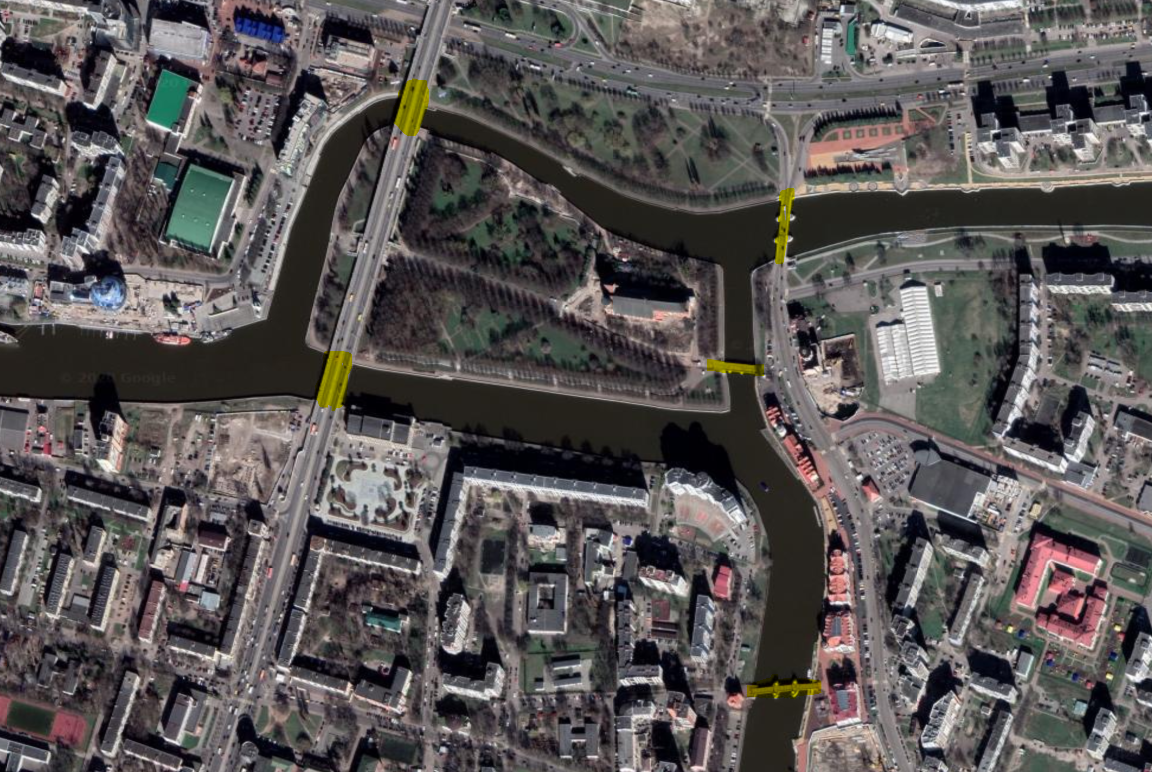
\includegraphics[height=3in]{ModernKonigsberg}
\end{center}
Is there an Euler path and/or circuit through this part of the city?  If so, find one.

\sol
First, we need to abstract this map with a graph, keeping the nodes in the same positions as before, but redrawing the edges to match the current bridges:
\begin{center}
\begin{tikzpicture}
  \GraphInit[vstyle=simple]
  \tikzset{VertexStyle/.append style={scale=0.3}}
  \SetGraphUnit{0.9}
  \Vertex{1}
  \NOWE(1){2}
  \SOWE(1){4}
  \WE(1){3}
  \Edge(1)(2)
  \Edge(1)(3)
  \Edge(1)(4)
  \Edge(2)(3)
  \Edge(3)(4)
  
  \extralabel{1}{0}{$a$}
  \extralabel{2}{90}{$b$}
  \extralabel{3}{180}{$c$}
  \extralabel{4}{-90}{$d$}
\end{tikzpicture}
\end{center}

Next, we can find the degree of each node:
\begin{center}
\begin{tikzpicture}
  \GraphInit[vstyle=simple]
  \tikzset{VertexStyle/.append style={scale=0.3}}
  \SetGraphUnit{0.9}
  \Vertex{1}
  \NOWE(1){2}
  \SOWE(1){4}
  \WE(1){3}
  \Edge(1)(2)
  \Edge(1)(3)
  \Edge(1)(4)
  \Edge(2)(3)
  \Edge(3)(4)
  
  \extralabel{1}{0}{$a$}
  \extralabel{2}{90}{$b$}
  \extralabel{3}{180}{$c$}
  \extralabel{4}{-90}{$d$}
  \extralabel{1}{45}{\color{red}3}
  \extralabel{2}{45}{\color{red}2}
  \extralabel{3}{135}{\color{red}3}
  \extralabel{4}{-45}{\color{red}2}
\end{tikzpicture}
\end{center}

Since there are exactly two odd nodes, it is possible to find an Euler path through this graph, but not an Euler circuit.  One Euler path is shown below:
\begin{center}
\begin{tikzpicture}
  \GraphInit[vstyle=simple]
  \tikzset{VertexStyle/.append style={scale=0.3}}
  \SetGraphUnit{0.9}
  \Vertex{1}
  \NOWE(1){2}
  \SOWE(1){4}
  \WE(1){3}
  
  \extralabel{1}{0}{$a$}
  \extralabel{2}{90}{$b$}
  \extralabel{3}{180}{$c$}
  \extralabel{4}{-90}{$d$}
  
  \tikzset{EdgeStyle/.append style={color=red}}
  \tikzstyle{LabelStyle}=[color=red,fill=white]
  \Edge[label=1](1)(2)
  \Edge[label=3](1)(3)
  \Edge[label=4](1)(4)
  \Edge[label=2](2)(3)
  \Edge[label=5](3)(4)
\end{tikzpicture}
\end{center}
This path can be written $\boxed{a \to b \to c \to a \to d \to c}$.  Notice that it starts at one of the odd nodes and ends at the other.
\end{example}
\pagebreak

\begin{example}[https://www.youtube.com/watch?v=Lr596-_L0M0&list=PLfmpjsIzhztst_PxJXo574wshSwxU9Yg_&index=4]{Existence of Euler Paths}
For each of the following graphs, determine if an Euler circuit exists.  If not, determine whether there is an Euler path.
\begin{center}
\begin{tabular}{c c c}
\begin{tikzpicture}
  \GraphInit[vstyle=simple]
  \tikzset{VertexStyle/.append style={scale=0.3}}
  \SetGraphUnit{0.5}
  \Vertex{1}
  \SOWE(1){3}
  \SOEA(1){4}
  \NOEA(4){2}
  \SOEA(2){5}
  \SOEA(3){6}
  \SOEA(4){7}
  
  \extralabel{1}{90}{$a$}
  \extralabel{2}{90}{$b$}
  \extralabel{3}{180}{$c$}
  \extralabel{4}{90}{$d$}
  \extralabel{5}{0}{$e$}
  \extralabel{6}{-90}{$f$}
  \extralabel{7}{-90}{$g$}
  
  \Edge(1)(2)
  \Edge(1)(3)
  \Edge(1)(4)
  \Edge(2)(4)
  \Edge(2)(5)
  \Edge(3)(4)
  \Edge(4)(5)
  \Edge(3)(6)
  \Edge(4)(6)
  \Edge(4)(7)
  \Edge(5)(7)
  \Edge(6)(7)
\end{tikzpicture}
&
\begin{tikzpicture}
  \GraphInit[vstyle=simple]
  \tikzset{VertexStyle/.append style={scale=0.3}}
  \SetGraphUnit{1}
  \Vertex{a}
  \EA(a){b}
  \SO(a){c}
  \SO(b){d}
  
  \extralabel{a}{90}{$a$}
  \extralabel{b}{90}{$b$}
  \extralabel{c}{-90}{$c$}
  \extralabel{d}{-90}{$d$}
  
  \Edge(a)(b)
  \Edge(a)(c)
  \Edge(b)(c)
  \SetUpEdge[style={bend right=30}]
  \Edge(b)(d)
  \Edge(d)(b)
  \Edge(c)(d)
  \Edge(d)(c)
\end{tikzpicture}
&
\begin{tikzpicture}[scale=0.65]
  \GraphInit[vstyle=simple]
  \tikzset{VertexStyle/.append style={scale=0.3}}
  \Vertex[x=0,y=0]{a}
  \Vertex[x=2.5,y=1]{b}
  \Vertex[x=6,y=1.2]{c}
  \Vertex[x=3.5,y=0.4]{d}
  \Vertex[x=2,y=-2]{e}
  \Vertex[x=4,y=-1.4]{f}
  \Vertex[x=7,y=-1.7]{g}
  \Vertex[x=0.5,y=-3]{h}
  \Vertex[x=3.5,y=-2.6]{i}
  \Vertex[x=6,y=-2.8]{j}
  
  \extralabel{a}{90}{$a$}
  \extralabel{b}{90}{$b$}
  \extralabel{c}{0}{$c$}
  \extralabel{d}{0}{$d$}
  \extralabel{e}{180}{$e$}
  \extralabel{f}{90}{$f$}
  \extralabel{g}{90}{$g$}
  \extralabel{h}{-90}{$h$}
  \extralabel{i}{-90}{$i$}
  \extralabel{j}{-90}{$j$}
  
  \Edge(a)(b)
  \Edge(a)(d)
  \Edge(a)(e)
  \Edge(a)(h)
  \Edge(b)(c)
  \Edge(b)(d)
  \Edge(b)(e)
  \Edge(b)(f)
  \Edge(b)(i)
  \Edge(c)(d)
  \Edge(c)(f)
  \Edge(c)(j)
  \Edge(d)(e)
  \Edge(d)(j)
  \Edge(d)(i)
  \Edge(e)(h)
  \Edge(e)(i)
  \Edge(e)(j)
  \Edge(f)(g)
  \Edge(f)(h)
  \Edge(g)(i)
  \Edge(g)(j)
  \Edge(h)(i)
  \Edge(i)(j)
  \Loop[dist=1cm,dir=NO,style={-}](c)
\end{tikzpicture}\\
& & \\
(a) & (b) & (c)
\end{tabular}
\end{center}

\sol
\begin{enumerate}[(a)]
\item Since all the nodes except $d$ are odd, each with a degree of 3, \boxtext{there is no Euler path or circuit} in this graph.
\item All the nodes in this graph are even ($a$ has degree 2, the rest have degree 4), \boxtext{there is an Euler circuit} for this graph.
\item Counting the degrees of each node for this graph is a bit more tedious, but the principle is the same.  The results are below (remember that a loop contributes 2 to the degree of its node):
\begin{center}
\begin{tabular}{c c}
\textbf{Node} & \textbf{Degree}\\
\hline
& \\
$a$ & 4\\
$b$ & 6\\
$c$ & 6\\
$d$ & 6\\
$e$ & 6\\
$f$ & 4\\
$g$ & 3\\
$h$ & 4\\
$i$ & 6\\
$j$ & 5
\end{tabular}
\end{center}
Since there are exactly two nodes ($g$ and $j$) with odd degree, \boxtext{there is an Euler path (but not an Euler circuit)} for this graph.
\end{enumerate}
\end{example}

\begin{try}[http://hartleymath.com/versatilemath/tryit/\#/graph-theory--euler-paths]
For each of the following graphs, determine if an Euler circuit exists.  If not, determine whether there is an Euler path.
\begin{center}
\begin{tabular}{c c}
\begin{tikzpicture}
  \GraphInit[vstyle=simple]
  \tikzset{VertexStyle/.append style={scale=0.3}}
  \grEmptyCycle[prefix=a,RA=1.5]{5}
  \Edge(a0)(a1)
  \Edge(a1)(a2)
  \Edge(a2)(a3)
  \Edge(a3)(a4)
  \Edge(a4)(a0)
  \Edge(a1)(a3)
  \Edge(a2)(a4)
\end{tikzpicture}
\hspace*{0.25in}
&
\hspace*{0.25in}
\begin{tikzpicture}
  \GraphInit[vstyle=simple]
  \tikzset{VertexStyle/.append style={scale=0.3}}
  \grComplete[RA=1.5]{5}
\end{tikzpicture}\\
& \\
(a) 
\hspace*{0.25in}
&
\hspace*{0.25in}
(b)
\end{tabular}
\end{center}
\end{try}
\pagebreak

\begin{example}[https://www.youtube.com/watch?v=tBkGIznLGZo&list=PLfmpjsIzhztst_PxJXo574wshSwxU9Yg_&index=5]{Euler Path through House}
The floor plan below shows the first floor of a single-family home.  Is there an Euler circuit/path through the interior of this level, using the highlighted doors (in other words, ignoring external doors and stairs)?
\begin{center}
\includegraphics[width=0.8\textwidth]{Sample_Floorplan}
\end{center}

\sol
First, let's draw a graph to represent this home, with each node representing a room and each edge representing a door.  Since the entrance is the most central location (in terms of connections to the rest of the home, we'll place that in the center, with edges out to the other rooms:
\begin{center}
\begin{tikzpicture}
\GraphInit[vstyle=simple]
  \tikzset{VertexStyle/.append style={scale=0.3}}
  \SetGraphUnit{2}
  \Vertex{ent}
  \EA(ent){fam}
  \NOEA(ent){liv}
  \NO(ent){kit}
  \NOWE(ent){pan}
  \WE(ent){lau}
  \SOWE(ent){bat}
  
  \extralabel{ent}{-45}{Entrance}
  \extralabel{fam}{-45}{Family Room}
  \extralabel{liv}{45}{Living/Dining}
  \extralabel{kit}{90}{Kitchen}
  \extralabel{pan}{90}{Pantry}
  \extralabel{lau}{180}{Laundry}
  \extralabel{bat}{-90}{Bathroom}
  
  \Edge(ent)(fam)
  \Edge(ent)(kit)
  \Edge(ent)(pan)
  \Edge(ent)(lau)
  \Edge(fam)(liv)
  \Edge(liv)(kit)
  
  \SetUpEdge[style={bend right=30}]
  \Edge(ent)(bat)
  \Edge(bat)(ent)
\end{tikzpicture}
\end{center}

Now, we can count the degree of each node:
\begin{center}
\begin{tabular}{l c}
\textbf{Room} & \textbf{Degree}\\
\hline
& \\
Entrance & 6\\
Family Room & 2\\
Living/Dining Room & 2\\
Kitchen & 2\\
Pantry & 1\\
Laundry & 1\\
Bathroom & 2
\end{tabular}
\end{center}

Since there are two rooms with an odd number of doors, \boxtext{there is an Euler path, but not an Euler circuit} through this level.  Any Euler path must start in either the pantry or laundry room and end in the other.
\end{example}
\pagebreak

\subsection{Finding an Euler Circuit}
It's fairly simple to determine whether or not an Euler circuit exists, by simply identifying the degree of each node.  Once we know that there \emph{is} such a circuit, it is often simple enough to find what it is just by looking at the graph and tracing through it, as long as the graph is relatively small.

However, here we'll illustrate a more systematic process for finding an Euler circuit, in case it is useful.  We'll use the graph below as an example.
\begin{center}
\begin{tikzpicture}[scale=0.7]
  \GraphInit[vstyle=simple]
  \tikzset{VertexStyle/.append style={scale=0.3}}
  \Vertex[x=0,y=0]{a}
  \Vertex[x=1,y=-2]{b}
  \Vertex[x=0,y=-4]{c}
  \Vertex[x=2,y=-3]{d}
  \Vertex[x=2,y=-1]{e}
  \Vertex[x=5,y=-2]{f}
  \Vertex[x=8,y=-3]{g}
  \Vertex[x=9,y=-2]{h}
  \Vertex[x=8,y=-1]{i}
  \Vertex[x=10,y=0]{j}
  \Vertex[x=10,y=-4]{k}
  
  \extralabel{a}{135}{$a$}
  \extralabel{b}{180}{$b$}
  \extralabel{c}{225}{$c$}
  \extralabel{d}{-90}{$d$}
  \extralabel{e}{90}{$e$}
  \extralabel{f}{90}{$f$}
  \extralabel{g}{-90}{$g$}
  \extralabel{h}{0}{$h$}
  \extralabel{i}{90}{$i$}
  \extralabel{j}{45}{$j$}
  \extralabel{k}{-45}{$k$}
  
  \SetUpEdge[style={bend right=20}]
  \Edge(a)(b)
  \Edge(b)(c)
  \Edge(a)(e)
  \Edge(d)(c)
  \Edge(e)(b)
  \Edge(b)(d)
  \Edge(d)(g)
  \Edge(i)(e)
  \Edge(g)(h)
  \Edge(h)(i)
  \Edge(i)(j)
  \Edge(h)(j)
  \Edge(k)(h)
  \Edge(k)(g)
  \SetUpEdge[style={bend right=10}]
  \Edge(e)(f)
  \Edge(f)(d)
  \Edge(f)(i)
  \Edge(g)(f)
\end{tikzpicture}
\end{center}

Notice that all the nodes are even, so it is possible to find an Euler circuit (or many, indeed).  We can start at any point, and eventually come back and end at the same node.

To begin, pick a starting point, and construct \textbf{\emph{any}} circuit through the graph.  Let's say we start with $a$; we could do something as simple as $a \to b \to e \to a$, but the longer our initial circuit is, the faster this process will go, so let's start with $a \to b \to c \to d \to b \to e \to a$:
\begin{center}
\begin{tikzpicture}[scale=0.7]
  \GraphInit[vstyle=simple]
  \tikzset{VertexStyle/.append style={scale=0.3}}
  \Vertex[x=0,y=0]{a}
  \Vertex[x=1,y=-2]{b}
  \Vertex[x=0,y=-4]{c}
  \Vertex[x=2,y=-3]{d}
  \Vertex[x=2,y=-1]{e}
  \Vertex[x=5,y=-2]{f}
  \Vertex[x=8,y=-3]{g}
  \Vertex[x=9,y=-2]{h}
  \Vertex[x=8,y=-1]{i}
  \Vertex[x=10,y=0]{j}
  \Vertex[x=10,y=-4]{k}
  
  \extralabel{a}{135}{$a$}
  \extralabel{b}{180}{$b$}
  \extralabel{c}{225}{$c$}
  \extralabel{d}{-90}{$d$}
  \extralabel{e}{90}{$e$}
  \extralabel{f}{90}{$f$}
  \extralabel{g}{-90}{$g$}
  \extralabel{h}{0}{$h$}
  \extralabel{i}{90}{$i$}
  \extralabel{j}{45}{$j$}
  \extralabel{k}{-45}{$k$}
  
  \SetUpEdge[style={bend right=20}]
  \Edge(d)(g)
  \Edge(i)(e)
  \Edge(g)(h)
  \Edge(h)(i)
  \Edge(i)(j)
  \Edge(h)(j)
  \Edge(k)(h)
  \Edge(k)(g)
  \SetUpEdge[style={bend right=10}]
  \Edge(e)(f)
  \Edge(f)(d)
  \Edge(f)(i)
  \Edge(g)(f)
  \SetUpEdge[style={bend right=20,color=blue!60!black}]
  \tikzstyle{LabelStyle}=[color=blue!60!black,fill=white]
  \Edge[label=1](a)(b)
  \Edge[label=2](b)(c)
  \Edge[label=6](a)(e)
  \Edge[label=3](d)(c)
  \Edge[label=5](e)(b)
  \Edge[label=4](b)(d)
\end{tikzpicture}
\end{center}

Now, delete those edges from the graph, and remove any points that are left isolated (so for instance, $a$ will be deleted, but $e$ will not, because there will be some remaining edges connected to $e$).
\begin{center}
\begin{tikzpicture}[scale=0.7]
  \GraphInit[vstyle=simple]
  \tikzset{VertexStyle/.append style={scale=0.3}}
  \Vertex[x=2,y=-3]{d}
  \Vertex[x=2,y=-1]{e}
  \Vertex[x=5,y=-2]{f}
  \Vertex[x=8,y=-3]{g}
  \Vertex[x=9,y=-2]{h}
  \Vertex[x=8,y=-1]{i}
  \Vertex[x=10,y=0]{j}
  \Vertex[x=10,y=-4]{k}
  
  \extralabel{d}{-90}{$d$}
  \extralabel{e}{90}{$e$}
  \extralabel{f}{90}{$f$}
  \extralabel{g}{-90}{$g$}
  \extralabel{h}{0}{$h$}
  \extralabel{i}{90}{$i$}
  \extralabel{j}{45}{$j$}
  \extralabel{k}{-45}{$k$}
  
  \SetUpEdge[style={bend right=20}]
  \Edge(d)(g)
  \Edge(i)(e)
  \Edge(g)(h)
  \Edge(h)(i)
  \Edge(i)(j)
  \Edge(h)(j)
  \Edge(k)(h)
  \Edge(k)(g)
  \SetUpEdge[style={bend right=10}]
  \Edge(e)(f)
  \Edge(f)(d)
  \Edge(f)(i)
  \Edge(g)(f)
\end{tikzpicture}
\end{center}

Then pick another point (we'll use $e$) and repeat this process.  Say, for instance, we pick the next circuit to be $e \to i \to f \to d \to g \to f \to e$:
\begin{center}
\begin{tikzpicture}[scale=0.7]
  \GraphInit[vstyle=simple]
  \tikzset{VertexStyle/.append style={scale=0.3}}
  \Vertex[x=2,y=-3]{d}
  \Vertex[x=2,y=-1]{e}
  \Vertex[x=5,y=-2]{f}
  \Vertex[x=8,y=-3]{g}
  \Vertex[x=9,y=-2]{h}
  \Vertex[x=8,y=-1]{i}
  \Vertex[x=10,y=0]{j}
  \Vertex[x=10,y=-4]{k}
  
  \extralabel{d}{-90}{$d$}
  \extralabel{e}{90}{$e$}
  \extralabel{f}{90}{$f$}
  \extralabel{g}{-90}{$g$}
  \extralabel{h}{0}{$h$}
  \extralabel{i}{90}{$i$}
  \extralabel{j}{45}{$j$}
  \extralabel{k}{-45}{$k$}
  
  \SetUpEdge[style={bend right=20}]
  \Edge(g)(h)
  \Edge(h)(i)
  \Edge(i)(j)
  \Edge(h)(j)
  \Edge(k)(h)
  \Edge(k)(g)
  \SetUpEdge[style={bend right=20,color=green!50!black}]
  \tikzstyle{LabelStyle}=[color=green!50!black,fill=white]
  \Edge[label=4](d)(g)
  \Edge[label=1](i)(e)
  \SetUpEdge[style={bend right=10,color=green!50!black}]
  \tikzstyle{LabelStyle}=[color=green!50!black,fill=white]
  \Edge[label=6](e)(f)
  \Edge[label=3](f)(d)
  \Edge[label=2](f)(i)
  \Edge[label=5](g)(f)
\end{tikzpicture}
\end{center}

After removing those edges and isolated points, we can find one final circuit through the remaining points: $i \to j \to h \to k \to g \to h \to i$:
\begin{center}
\begin{tikzpicture}[scale=0.7]
  \GraphInit[vstyle=simple]
  \tikzset{VertexStyle/.append style={scale=0.3}}
  \Vertex[x=8,y=-3]{g}
  \Vertex[x=9,y=-2]{h}
  \Vertex[x=8,y=-1]{i}
  \Vertex[x=10,y=0]{j}
  \Vertex[x=10,y=-4]{k}
  
  \extralabel{g}{-90}{$g$}
  \extralabel{h}{0}{$h$}
  \extralabel{i}{90}{$i$}
  \extralabel{j}{45}{$j$}
  \extralabel{k}{-45}{$k$}
  
  \SetUpEdge[style={bend right=20,color=red!80!black}]
  \tikzstyle{LabelStyle}=[color=red!80!black,fill=white]
  \Edge[label=5](g)(h)
  \Edge[label=6](h)(i)
  \Edge[label=1](i)(j)
  \Edge[label=2](h)(j)
  \Edge[label=3](k)(h)
  \Edge[label=4](k)(g)
\end{tikzpicture}
\end{center}

Having used all the edges now, we have three partial circuits:
\begin{center}
{\color{blue!60!black}$a \to b \to c \to d \to b \to e \to a$}\\
{\color{green!50!black}$e \to i \to f \to d \to g \to f \to e$}\\
{\color{red!80!black}$i \to j \to h \to k \to g \to h \to i$}
\end{center}

To construct the final Euler circuit through the full graph, we simply stitch these three circuits together.  Start from the end: notice that the last one begins and ends with $i$.  Then, go to the one just before that: when that second circuit passes through $i$, we can pause and run through the third circuit before resuming.  In practice, just replace $i$ with the third circuit; instead of 
\begin{center}
{\color{green!50!black}$e \to i \to f \to d \to g \to f \to e$}
\end{center}
we will now have
\begin{center}
{\color{green!50!black}$e \to$} {\color{red!80!black}$i \to j \to h \to k \to g \to h \to i$} {\color{green!50!black}$\to f \to d \to g \to f \to e$}
\end{center}

Finally, notice that this long string begins and ends at $e$, so we can substitute the whole thing in the place of $e$ in the first circuit, and we'll have our full Euler circuit:
\begin{center}
{\color{blue!60!black}$a \to b \to c \to d \to b \to$} {\color{green!50!black}$e \to$} {\color{red!80!black}$i \to j \to h \to k \to g \to h \to i$} {\color{green!50!black}$\to f \to d \to g \to f \to e$} {\color{blue!60!black}$\to a$}
\end{center}

Again, in many cases there's no need to resort to a systematic process like this, but if you have trouble spotting an Euler circuit immediately, you can try it.

\subsection{Euler Paths in Directed Graphs}
The rule we described earlier (all nodes even $\to$ Euler circuit; two odd nodes $\to$ Euler path) applies to \emph{undirected} graphs, but what about directed graphs?  Now we don't have a single degree for each node; they each have an in-degree and an out-degree.  Can we develop a similar rule, though?\\

With a bit of thought, we can adapt the earlier rule for directed graphs.  Specifically, think about the condition for an Euler circuit, that all nodes be even.  What does this actually mean?  The reason for this is that we need to be able to leave every node that we arrive at, so really what the rule implies is that there are as many ways out as ways in.  Thinking about it that way makes it clear that for a directed graph, we will look to see whether the in-degree and out-degree are equal.\\

Similarly, the condition for an Euler path is really about verifying that only the starting and ending node have one more exit and entrance, respectively, than the others, which all have equal entrances and exits.  So for a directed graph, we can adapt this condition to say that all the nodes should have equal in-degree and out-degree, except for two: one of which has one more inlet than outlet, and the other has one more outlet than inlet.
\pagebreak

\begin{formula}{Euler Paths in Directed Graphs}
If each node of a directed graph has equal in-degree and out-degree, the graph has an Euler circuit.\\

If one node has an in-degree that is larger than its out-degree by 1, and another node has an out-degree that is larger than its in-degree by 1, there is no Euler circuit, but there is an Euler path (starting at the node with larger out-degree and ending at the node with larger in-degree).
\end{formula}

\begin{example}[https://www.youtube.com/watch?v=2N7o_CWptpM&list=PLfmpjsIzhztst_PxJXo574wshSwxU9Yg_&index=6]{Euler Paths in Directed Graphs}
For each of the following graphs, determine if an Euler circuit exists.  If not, determine whether there is an Euler path.
\begin{center}
\begin{tabular}{c c}
\begin{tikzpicture}
  \GraphInit[vstyle=simple]
  \tikzset{VertexStyle/.append style={scale=0.3}}
  \SetGraphUnit{2.2}
  \Vertex{a}
  \EA(a){b}
  \SO(a){c}
  \SO(b){d}
  
  \extralabel{a}{90}{$a$}
  \extralabel{b}{90}{$b$}
  \extralabel{c}{-90}{$c$}
  \extralabel{d}{-90}{$d$}
  
  \tikzset{EdgeStyle/.style = {->-,>=latex[round]}}
  \Edge(a)(b)
  \Edge(c)(a)
  \Edge(b)(c)
  \Edge(a)(d)
  \tikzset{EdgeStyle/.style = {->-,>=latex[round],bend right=20}}
  \Edge(c)(d)
  \Edge(d)(c)
  \Edge(b)(d)
  \Edge(d)(b)
\end{tikzpicture}
\hspace*{0.2in}
&
\hspace*{0.2in}
\begin{tikzpicture}
  \GraphInit[vstyle=simple]
  \tikzset{VertexStyle/.append style={scale=0.3}}
  \SetGraphUnit{2.2}
  \Vertex{a}
  \EA(a){b}
  \SO(a){c}
  \SO(b){d}
  \EA(b){e}
  
  \extralabel{a}{90}{$a$}
  \extralabel{b}{90}{$b$}
  \extralabel{c}{-90}{$c$}
  \extralabel{d}{-90}{$d$}
  \extralabel{e}{90}{$e$}
  
  \tikzset{EdgeStyle/.style = {->-,>=latex[round]}}
  \Edge(a)(c)
  \Edge(b)(a)
  \Edge(e)(b)
  \Edge(d)(e)
  \Edge(c)(d)
  \tikzset{EdgeStyle/.style = {->-,>=latex[round],bend right=20}}
  \Edge(b)(d)
  \Edge(d)(b)
  \Edge(c)(b)
  \Edge(b)(c)
\end{tikzpicture}\\
& \\
(a) \hspace*{0.2in} & \hspace*{0.2in} (b)
\end{tabular}
\end{center}

\sol
\begin{enumerate}[(a)]
\item Count the in-degree and out-degree of each node:
\begin{center}
\begin{tabular}{c c c}
\textbf{Node} & \textbf{In-Degree} & \textbf{Out-Degree}\\
\hline
 & & \\
$a$ & 1 & 2\\
$b$ & 2 & 2\\
$c$ & 2 & 2\\
$d$ & 3 & 2
\end{tabular}
\end{center}
Notice that only two nodes do not have equal in- and out-degrees; one of them has exactly one more outlet than inlet, and the other has the reverse.  Thus, \boxtext{while there is no Euler circuit, there is an Euler path} for this graph, starting at $a$ and ending at $d$.

\item Again, count the degrees:
\begin{center}
\begin{tabular}{c c c}
\textbf{Node} & \textbf{In-Degree} & \textbf{Out-Degree}\\
\hline
 & & \\
$a$ & 1 & 1\\
$b$ & 3 & 3\\
$c$ & 2 & 2\\
$d$ & 2 & 2\\
$e$ & 1 & 1
\end{tabular}
\end{center}
This time, all the nodes have equal in-degree and out-degree, so \boxtext{there is an Euler circuit} for this graph (we could start at any node).
\end{enumerate}
\end{example}
\vfill
\pagebreak

\def\icosianpuzzlesidenote{\marginnote{Although William Rowan Hamilton was not the first one to study these paths, they are named for him because he invented a puzzle called the Icosian game, which starts with a 12-sided \emph{dodecahedron}:
\begin{center}
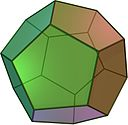
\includegraphics[width=0.75in]{dodecahedron}
\end{center}
The goal is to find a Hamilton circuit, traveling along the edges and touching each corner exactly once.  Hamilton sold this puzzle to a game dealer, and it was marketed throughout Europe.  In the most popular form, the dodecahedron was modeled as a planar graph, like this one:
\begin{center}
\begin{tikzpicture}[scale=0.5]
  \GraphInit[vstyle=simple]
  \tikzset{VertexStyle/.append style={scale=0.3}}
  \grEmptyCycle[prefix=a,RA=3,rotation=18]{5}
  \grEmptyCycle[prefix=b,RA=2,rotation=18]{5}
  \grEmptyCycle[prefix=c,RA=1.3,rotation=198]{5}
  \grEmptyCycle[prefix=d,RA=0.7,rotation=198]{5}
  
  \Edge(a0)(a1)
  \Edge(a3)(a4)
  \Edge(d2)(d3)
  \Edge(d4)(d0)
  
  \Edge(a2)(b2)
  \Edge(c1)(d1)
  
  \Edge(b0)(c3)
  \Edge(b1)(c4)
  \Edge(b3)(c0)
  \Edge(b4)(c2)
  
  \SetUpEdge[style={color=red}]
  \Edge(a1)(a2)
  \Edge(a2)(a3)
  \Edge(a4)(a0)
  \Edge(d1)(d2)
  \Edge(d0)(d1)
  \Edge(d3)(d4)
  
  \Edge(a3)(b3)
  \Edge(b4)(c1)
  \Edge(a4)(b4)
  \Edge(a0)(b0)
  \Edge(c2)(d2)
  \Edge(c0)(d0)
  \Edge(c4)(d4)
  \Edge(c3)(d3)
  \Edge(a1)(b1)
  
  \Edge(b3)(c1)
  \Edge(b0)(c2)
  \Edge(b2)(c0)
  \Edge(b2)(c4)
  \Edge(b1)(c3)
\end{tikzpicture}
\end{center}

It was sold as a wooden board with pegs at the nodes of the graph, and players would wind a string along a path to solve it (one solution is shown in red).  %Often the pegs would be labeled with the names of 20 cities, so that players could imagine plotting a journey.
}}

\subsection{Hamilton Paths}
Take a look at the map below; what do you see?
\begin{center}
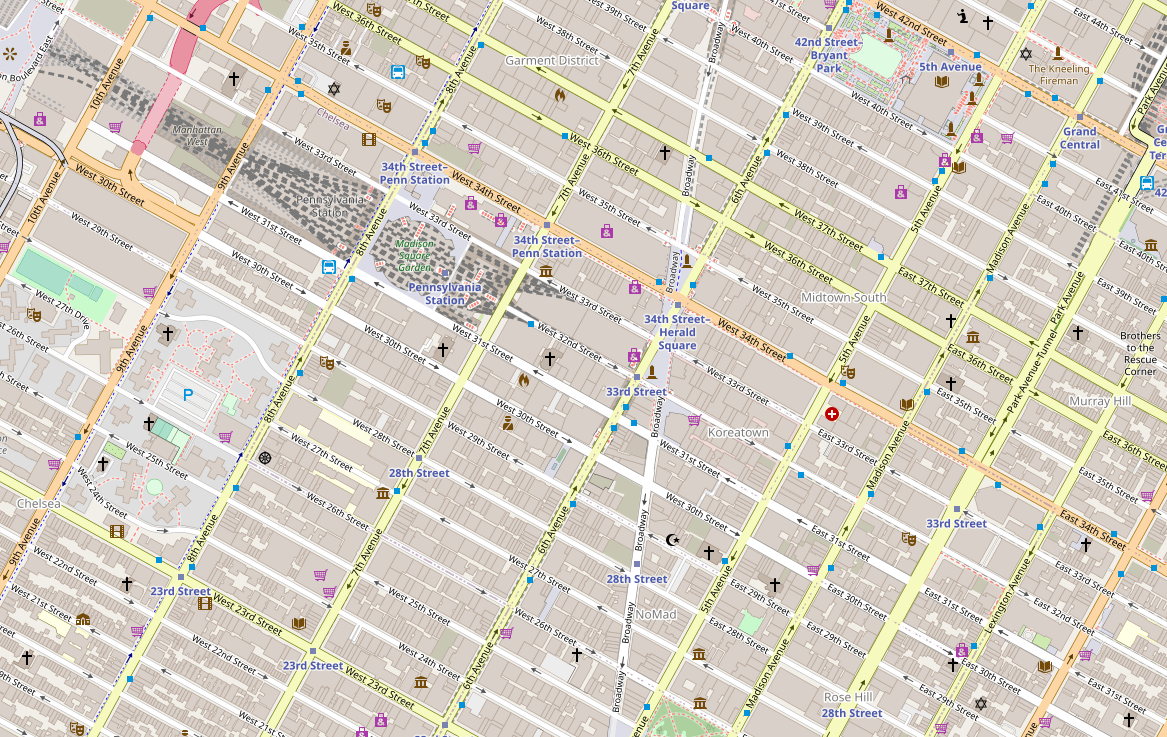
\includegraphics[width=0.6\textwidth]{citygrid}
\end{center}

By now, you can probably see a graph; if we designate each intersection as a node, the edges would be one-block segments of streets.\\

Now, suppose you work for the city's public works department, and your job is to schedule workers throughout the city as efficiently as possible.

After a snowstorm, your job is plan routes for the snowplows to get the streets cleared with a minimal amount of wasted driving.  This is, in fact, an Euler path problem (or more likely a Chinese Postman problem, if an Euler path doesn't exist).  Having read this chapter, you draw up a hyper-efficient plan and save the city thousands in fuel.\\

A\icosianpuzzlesidenote\ few months later, the city decides to switch out all the traffic lights for a new, more efficient, more reliable model.  Since you did such a great job with the snowplow scheduling, the department tasks you with planning the routes of the work crews through the city for this new contract.  What's different about this problem?

In the snowplow problem, the goal was to \emph{travel along every \textbf{edge}} exactly once.  Now, with the traffic light problem, the edges are not the important part: there's no need to drive along every road, but simply to reach every intersection so that the crew can do their work there.  Thus, the goal of the traffic light problem is to \emph{travel to every \textbf{node}} exactly once.  This is an entirely new kind of problem, and what we're looking for now is called a \textbf{Hamilton path}.

\begin{formula}{Hamilton Paths}
A \textbf{Hamilton path} (or Hamiltonian path) in a graph is a path that passes through every node of the graph exactly once (and a Hamilton circuit is a Hamilton path that happens to be a circuit).
\end{formula}

Now, having seen how easy it is to determine whether a graph has an Euler path or circuit, you may be expecting a similar rule for Hamilton paths.  However, it turns out that there is no known rule that can tell us for certain whether or not any graph has a Hamilton path or circuit.

There are a few observations that we can make:
\begin{enumerate}
\item Every complete graph has a Hamilton path, and as long as there are at least 3 nodes, there is a Hamilton circuit.  Since there are edges between every pair of nodes, we can visit all the nodes in any order we choose.
\item If a graph has a node with degree 1, it cannot have a Hamilton circuit, because there's no way to both arrive at and leave that node.  It could, of course, have a Hamilton path.
\item When drawing a Hamilton path/circuit, once you have marked a node, you can eliminate all the other edges that connect to that node, which can simplify the picture.
\end{enumerate}

There are other, more complicated theorems that give conditions under which Hamilton circuits exist (for instance, \emph{Dirac's Theorem} says that a simple graph with $n$ nodes, where $n \geq 3$, has a Hamilton circuit if the degree of every node is at least half of $n$), but for our purposes, we will simply check whether a graph has a Hamilton path or circuit by inspecting it and seeing if we can find one.  Since we'll only deal with small graphs, this is good enough for us.  For larger graphs, we could use a \emph{brute force} approach, which means trying all the possible paths to see if any is Hamiltonian (as you can imagine, this is quite tedious).

\begin{example}[https://www.youtube.com/watch?v=fMz9k_Z2Trg&list=PLfmpjsIzhztst_PxJXo574wshSwxU9Yg_&index=7]{Hamilton Paths}
For each of the following graphs, determine whether a Hamilton circuit exists; if so, describe the circuit.  If there is no Hamilton circuit, see if there is a Hamilton path.
\begin{center}
\begin{tabular}{c c c}
\begin{tikzpicture}[scale=0.45]
  \GraphInit[vstyle=simple]
  \tikzset{VertexStyle/.append style={scale=0.3}}
  \SetGraphUnit{4}
  \Vertex{a}
  \EA(a){b}
  \SO(a){c}
  \EA(c){d}
  
  \extralabel{a}{90}{$a$}
  \extralabel{b}{90}{$b$}
  \extralabel{c}{-90}{$c$}
  \extralabel{d}{-90}{$d$}
  
  \Edge(a)(b)
  \Edge(a)(c)
  \Edge(a)(d)
  \Edge(b)(c)
  \Edge(b)(d)
  \Edge(c)(d)
\end{tikzpicture}
\hspace*{0.15in}
&
\hspace*{0.15in}
\begin{tikzpicture}[scale=0.35]
  \GraphInit[vstyle=simple]
  \tikzset{VertexStyle/.append style={scale=0.3}}
  \SetGraphUnit{3}
  \Vertex{a}
  \SOEA(a){c}
  \SOWE(c){b}
  \EA(c){f}
  \NOEA(f){d}
  \SOEA(f){e}
  
  \extralabel{a}{90}{$a$}
  \extralabel{b}{-90}{$b$}
  \extralabel{c}{90}{$c$}
  \extralabel{d}{90}{$d$}
  \extralabel{e}{-90}{$e$}
  \extralabel{f}{90}{$f$}
  
  \Edge(a)(b)
  \Edge(a)(c)
  \Edge(b)(c)
  \Edge(c)(f)
  \Edge(f)(d)
  \Edge(e)(f)
  \Edge(e)(d)
\end{tikzpicture}
\hspace*{0.15in}
&
\hspace*{0.15in}
\begin{tikzpicture}[scale=0.35]
  \GraphInit[vstyle=simple]
  \tikzset{VertexStyle/.append style={scale=0.3}}
  \SetGraphUnit{3}
  \Vertex{ent}
  \EA(ent){fam}
  \NOEA(ent){liv}
  \NO(ent){kit}
  \NOWE(ent){pan}
  \WE(ent){lau}
  \SOWE(ent){bat}
  
  \extralabel{ent}{-45}{$e$}
  \extralabel{fam}{-45}{$f$}
  \extralabel{liv}{45}{$c$}
  \extralabel{kit}{90}{$b$}
  \extralabel{pan}{90}{$a$}
  \extralabel{lau}{180}{$d$}
  \extralabel{bat}{-90}{$g$}
  
  \Edge(ent)(fam)
  \Edge(ent)(kit)
  \Edge(ent)(pan)
  \Edge(ent)(lau)
  \Edge(fam)(liv)
  \Edge(liv)(kit)
  
  \SetUpEdge[style={bend right=30}]
  \Edge(ent)(bat)
  \Edge(bat)(ent)
\end{tikzpicture}\\
(a) 
\hspace*{0.15in}
&
\hspace*{0.15in}
(b)
\hspace*{0.15in}
&
\hspace*{0.15in}
(c)
\end{tabular}
\end{center}

\sol
\begin{enumerate}[(a)]
\item Since this is a complete graph, $K_4$, we know that \boxtext{a Hamilton circuit exists}.  We could trace, for instance, the path $\boxed{a \to d \to c \to b}$.
\item There is no Hamilton circuit, because $c$ and $f$ form bottlenecks; once you pass through one of them to go to the other side of the graph, there's no way to return.  However, \boxtext{we can find a Hamilton path; $a \to b \to c \to d \to e \to f$, for instance}.

\item We know that there is no Hamilton circuit, because we have nodes with degree 1.  Let's look for a Hamilton path; say we start at $a$.  As soon as we travel to $e$, we're trapped, because no matter where we go, we'll cut off several points without any way to get to them without going back through $e$.  Therefore, \boxtext{there is no Hamilton circuit or path} for this graph.
\end{enumerate}
\end{example}

\begin{try}[http://hartleymath.com/versatilemath/tryit/\#/graph-theory--hamilton-paths]
For each of the following graphs, determine whether a Hamilton circuit exists; if so, describe the circuit.  If there is no Hamilton circuit, see if there is a Hamilton path.
\begin{center}
\begin{tabular}{c c c}
\begin{tikzpicture}[scale=0.45]
  \GraphInit[vstyle=simple]
  \tikzset{VertexStyle/.append style={scale=0.3}}
  \grCycle[RA=2.5,prefix=a]{5}
  
  \extralabel{a0}{0}{$a$}
  \extralabel{a1}{45}{$b$}
  \extralabel{a2}{135}{$c$}
  \extralabel{a3}{225}{$d$}
  \extralabel{a4}{-45}{$e$}
  
  \Edge(a1)(a3)
  \Edge(a2)(a4)
\end{tikzpicture}
\hspace*{0.2in}
&
\hspace*{0.2in}
\begin{tikzpicture}[scale=0.35]
  \GraphInit[vstyle=simple]
  \tikzset{VertexStyle/.append style={scale=0.3}}
  \SetGraphUnit{4}
  \Vertex{a}
  \EA(a){b}
  \EA(b){c}
  \SO(b){d}
  \WE(d){e}
  
  \extralabel{a}{90}{$a$}
  \extralabel{b}{90}{$b$}
  \extralabel{c}{90}{$c$}
  \extralabel{d}{-90}{$d$}
  \extralabel{e}{-90}{$e$}
  
  \Edge(a)(b)
  \Edge(a)(e)
  \Edge(b)(c)
  \Edge(b)(d)
  \Edge(b)(e)
  \Edge(c)(d)
  \Edge(d)(e)
\end{tikzpicture}\\
(a) 
\hspace*{0.2in}
&
\hspace*{0.2in}
(b)
\end{tabular}
\end{center}
\end{try}